\documentclass[a4paper,14pt]{extarticle} \usepackage[utf8]{inputenc}
\usepackage[T1]{fontenc}
\usepackage[margin=2.5cm]{geometry}

% Fonte Caladea se existir, senão lmodern
\IfFileExists{caladea.sty}{
  \usepackage{caladea}
}{
  \usepackage{lmodern} }
\usepackage{ragged2e}
\usepackage{graphicx}
\usepackage[portuguese]{babel}
\usepackage{wrapfig}
\usepackage{hyperref}
\usepackage{fancyhdr}
\usepackage{xcolor}
\usepackage{rotating}
\usepackage{titlesec}
\usepackage{epigraph}
\usepackage{dirtytalk}
\usepackage{indentfirst} % Indenta o primeiro parágrafo após seções

% Ajuste do recuo de parágrafo
\setlength{\parindent}{1.5em}

% Centralizar títulos
\titleformat{\section}
  {\normalfont\centering\bfseries\Large}{\thesection}{1em}{}

\titleformat{\subsection}
  {\normalfont\centering\bfseries\large}{\thesubsection}{1em}{}

\titleformat{\subsubsection}
  {\normalfont\centering\bfseries}{\thesubsubsection}{1em}{}

% -------------- Símbolos de Versículo e Resposta --------------
% Definição do símbolo (a “barrinha” inclinada)
\makeatletter
\newcommand{\vers@resp@sym}{%
  \raisebox{0.2ex}{\rotatebox[origin=c]{-20}{$\m@th\rceil$}}%
}
% macro interna que sobrepõe a barrinha e a letra V ou R
\newcommand{\vers@resp}[2]{%
  {\ooalign{%
     \hidewidth\kern#1\vers@resp@sym\hidewidth\cr
     #2\cr
  }}%
}
% comandos públicos \versicle e \response
\DeclareRobustCommand{\versicle}{\vers@resp{-0.1em}{V}}
\DeclareRobustCommand{\response}{\vers@resp{0pt}{R}}
\makeatother
% ^------------- Símbolos de Versículo e Resposta -------------^

% Rodapé com imagem e página
\pagestyle{fancy}
% ---- Cabeçalho ------------
\fancyhf[C]{}
% ----- Rodapé --------------
\fancyfoot[LO,LE]{%
  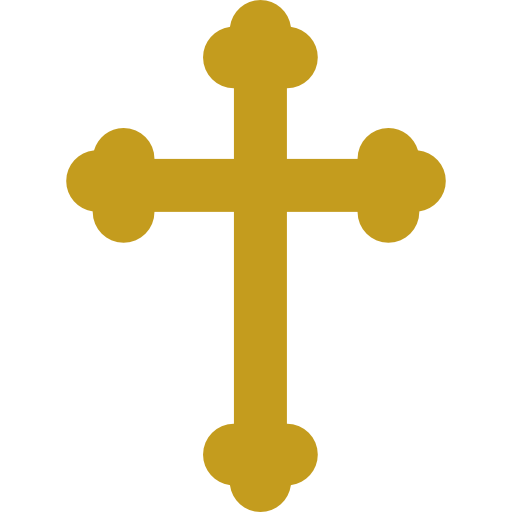
\includegraphics[scale=0.2]{assets/cross.png}\quad
  \textit{Novena a \textbf{São Moisés}}
}
\fancyfoot[RO,RE]{\thepage}

\begin{document}

\subsection*{Novena a São Moisés, Profeta}
Profeta, que Deus escolheu para libertar o seu povo do Egito e conduzi-lo à Terra Prometida. Segundo alguns estudiosos, Moisés, também quer dizer “aquele que salva” o seu povo.

\par\noindent\rule{\textwidth}{0.4pt}

\tableofcontents
\thispagestyle{empty}

% --- Vida / Origem da Novena ---
\newpage



\newpage

% --- Orações Diárias ---
\section{Novena de São Moisés}

\subsection{Oração Inicial}
Você ascendeu às alturas das virtudes, Profeta Moisés; portanto, foi considerado digno de ver a Glória de Deus. Tendo recebido as Tábuas da Lei cheias de Graça e carregando a Graça da escrita dentro de si, você foi o louvor honroso dos Profetas e um grande mistério de piedade.

O coro dos Profetas se alegra com Moisés e Arão hoje, pois o cumprimento de sua Profecia está entre nós. A Cruz, pela qual Tu nos salvaste, brilha hoje. 

Ó Cristo Deus, tem misericórdia de nós.



\subsection{1º Dia}
\textbf{Sugestão: Leitura do Livro do Êxodo (Êxodo 2,1-25):}

$^{1. }$Depois disto, um homem da família de Levi partiu e tomou para esposa uma mulher da sua estirpe.

$^{2. }$Ela concebeu e deu à luz um filho, e, vendo-o muito lindo, escondeu-o por espaço de três meses.

$^{3. }$Todavia não podendo mais tê-lo escondido, tomou um cesto de junco, barrou-lo com betume e pez, meteu dentro o menino e expô-lo num canavial junto da margem do rio,

$^{4. }$estando ao longe a sua irmã a observar o que (lhe) sucederia.

$^{5. }$A filha do Faraó veio lavar-se ao rio, e as suas donzelas caminhavam ao longo da margem. Tendo ela visto o cesto no canavial, mandou uma das suas criadas trazer-lho:

$^{6. }$abrindo-o, e vendo nele um menino que vagia, compadecida dele, disse: Este é um dos meninos dos hebreus.

$^{7. }$A irmã do menino disse-lhe: Queres que vá e que te chame uma mulher hebreia, que possa aleitar o menino?

$^{8. }$Ela respondeu: Vai. A donzela partiu e chamou sua mãe.

$^{9. }$E a filha de Faraó disse-lhe: Toma este menino e aleita-mo: eu te darei a paga. A mulher tomou, aleitou o menino, e, quando estava crescido, entregou-o à filha do Faraó,

$^{10. }$que o adoptou por filho, e pôs-lhe o nome de Moisés, dizendo: eu o tirei da água.

$^{11. }$Naqueles dias, sendo Moisés já grande, saiu a visitar seus irmãos e viu a sua aflição. Um dia reparou que um homem egípcio maltratava um dos hebreus seus irmãos.

$^{12. }$Tendo olhado para uma e outra parte, vendo que não estava ali ninguém, matou o egípcio e escondeu-o na areia.

$^{13. }$Saindo no dia seguinte, viu dois hebreus rixando, e disse ao agressor: Por que feres o teu próximo?

$^{14. }$Ele respondeu: Quem te constituiu principe e juiz sobre nós? Acaso queres tu matar-me, como mataste o egípcio? Moisés temeu e disse: Como é que tal coisa se descobriu?

$^{15. }$Faraó foi informado do acontecimento e procurava matar Moisés; ele, porém, fugindo da sua vista, parou na terra de Madian e assentou-se junto de um poço.

$^{16. }$Ora o sacerdote de Madian tinha sete filhas, as quais foram tirar água. Tendo enchido as pias, queriam dar de beber aos rebanhos de seu pai,

$^{17. }$mas sobrevieram os pastores e lançaram-nas fora dali. Moisés levantou-se, e, tomando a defesa das moças, deu de beber às suas ovelhas.

$^{18. }$Quando elas voltaram para casa de Raquel, seu pai, este disse-lhes: Por que viestes mais cedo do que o costume?

$^{19. }$Responderam: Um homem egipcio livrou-nos das mãos dos pastores, e, além disso, tirou água connosco e deu de beber às ovelhas.

$^{20. }$Ele disse: Onde está? Por que deixastes partir esse homem? Chamai-o para comer pão.

$^{21. }$Consentiu Moisés em ficar em casa dele, e tomou por mulher a Séfora, sua filha.

$^{22. }$Ela deu à luz um filho, a quem Moisés pôs o nome de Gersão, dizendo: Fui peregrino numa terra estrangeira.

$^{23. }$Muito tempo depois, porém, morreu o rei do Egipto. Os filhos de Israel, gemendo debaixo do peso dos trabalhos, clamaram, e o seu clamor, por causa dos trabalhos, subiu até Deus,

$^{24. }$o qual ouviu os seus gemidos, e se lembrou da aliança que tinha feito com Abraão, Isaac e Jacob.

$^{25. }$O Senhor olhou para os filhos de Israel e reconheceu-os (por seus filhos).

\par\noindent\rule{\textwidth}{0.4pt}

Palavra do Senhor. Graças a Deus.

Rezar a \textbf{\nameref{oracao-final}.}
\subsection{2º Dia}
\textbf{Sugestão: Leitura do Livro do Êxodo (Êxodo 3:1–10):}

$^{1.}$Ora Moisés apascentava as ovelhas de Jetro, seu sogro, sacerdote de Madian. Tendo conduzido o rebanho para o interior do deserto, chegou ao monte de Deus, a Horeb.

$^{2.}$O Senhor apareceu-lhe numa chama de fogo (que saia) do meio de uma sarça, e (Moisés) via que a sarça ardia sem se consumir.

$^{3.}$Disse, pois, Moisés: Irei examinar (de perto) esta grande visão, (e verei) por que causa se não consome a sarça.

$^{4.}$Porém o Senhor, vendo que ele se movia para ir ver, chamou-o do meio da sarça e disse: Moisés, Moisés. Ele respondeu: Aqui estou.

$^{5.}$E (o Senhor) disse; Não te aproximes daqui; tira as sandálias de teus pés, porque o lugar em que estás, é uma terra santa.

$^{6.}$E acrescentou: Eu sou o Deus de teu pai, o Deus de Abraão, o Deus de Isaac e o Deus de Jacob. Cobriu Moisés o rosto, porque não ousava olhar para Deus.

$^{7.}$O Senhor disse-lhe: Eu vi a aflição do meu povo no Egipto, ouvi o seu clamor causado pela crueza daqueles que têm a superintendência das obras.

$^{8.}$Conhecendo a sua dor, desceu para o livrar das mãos dos Egípcios e para o conduzir daquela terra para uma terra boa e espaçosa, para uma terra onde corre o leite e o mel, nas regiões do Cananeu, do Heteu, do Amorreu, do Ferezeu, do Heveu do Jebuseu.

$^{9.}$O clamor, pois, dos filhos de Israel chegou até mim, e eu vi a aflição com que são oprimidos pelos Egípcios.

$^{10.}$Mas vem e eu te enviarei a Faraó, a fim de que tires do Egipto o meu povo, os filhos de Israel.


\par\noindent\rule{\textwidth}{0.4pt}

Palavra do Senhor. Graças a Deus.

Rezar a \textbf{\nameref{oracao-final}.}
\subsection{3º Dia}
\textbf{Sugestão: Leitura do Livro do Êxodo (Êxodo 7:1–24):}

$^{1.}$O Senhor disse a Moisés: Repara que te constitui deus de Faraó; Aarão, teu irmão, será teu profeta. (ver nota)

$^{2.}$Tu lhe dirás tudo o que eu te mando, e ele falará a Faraó, para que deixe partir do seu país os filhos de Israel.

$^{3.}$Eu endurecerei o seu coração, e multiplicarei os meus sinais e os meus prodigios na terra do Egipto.

$^{4.}$Faraó não vos ouvirá, mas eu estenderei a minha mão sobre o Egipto e farei sair do Egipto o meu exército, o meu povo, os filhos de Israel, por meio dos maiores juízos.

$^{5.}$Os Egípcios saberão que eu sou o Senhor, quando eu estender a minha mão sobre o Egipto, e fizer sair do meio deles os filhos de Israel.

$^{6.}$Fizeram, pois, Moisés e Aarão como o Senhor tinha mandado; fizeram-no exactamente.

$^{7.}$Moisés tinha oitenta anos, e Aarão oitenta e três, quando falaram a Faraó.

$^{8.}$O Senhor disse a Moisés e a Aarão:

$^{9.}$Quando Faraó vos disser: Fazei um prodígio-tu dirás a Aarão: Pega na tua vara, lança-a por terra diante de Faraó, e ela se converterá em serpente.

$^{10.}$Tendo, pois, Moisés e Aarão ido à presença de Faraó, fizeram conforme o Senhor tinha ordenado: Aarão lançou por terra a vara diante de Faraó e dos seus servos, e ela converteu-se em serpente.

$^{11.}$Mas Faraó chamou os sábios e os magos, e eles fizeram também coisas semelhantes por meio dos encantamentos egípcios e de certos segredos.

$^{12.}$Lançaram por terra cada um deles as suas varas, as quais se converteram em dragões, mas a vara de Aarão devorou as varas deles. (ver nota)

$^{13.}$Endureceu-se o coração de Faraó e não os ouviu, como o Senhor tinha dito.

$^{14.}$O Senhor disse a Moisés: Obstinou-se o coração de Faraó; não quer deixar partir o (meu) povo.

$^{15.}$Vai ter com ele pela manhã. Ele sairá (para ir) ao rio, e tu estarás em frente dele sobre a margem do rio, tomarás na tua mão a vara, que se converteu em dragão,

$^{16.}$e lhe dirás: o Senhor Deus dos Hebreus enviou-me a ti para (te) dizer: Deixa sair o meu povo para que me ofereça sacrifícios no deserto. Até ao presente não quiseste ouvir.

$^{17.}$Olha, pois, o que diz o Senhor: Nisto conhecerás que eu sou o Senhor: ferirei com a vara, que tenho na minha mão, a água do rio e ela se converterá em sangue.

$^{18.}$Os peixes que há no rio morrerão, as águas se corromperão, e os Egípcios sentirão repugnância de a beber.

$^{19.}$O Senhor disse também a Moisés; Dize a Aarão: Toma a tua vara, e estende a tua mão sobre as águas do Egipto, sobre os seus rios, ribeiros, lagoas, e todos os reservatórios de águas, para que se convertam em sangue; e haverá sangue em toda a terra do Egipto, tanto nos vasos de madeira, como nos de pedra.

$^{20.}$Moisés e Aarão fizeram como o Senhor lhes mandará. (Aarão), levantando a vara, feriu a água do rio, na presença de Faraó e dos seus servos, e ela converteu-se em sangue.

$^{21.}$Os peixes, que havia no rio, morreram, e o rio, corrompeu-se, e os Egípcios não podiam beber da água do rio, e houve sangue por toda a terra do Egípto.

$^{22.}$Porém os magos do Egipto fizeram coisas semelhantes com os seus encantamentos, e o coração de Faraó endureceu-se, e não os ouviu, como o Senhor tinha predito. (ver nota)

$^{23.}$(Faraó) voltou-lhes as costas, entrou em sua casa e não aplicou o seu coração (a estas coisas) ainda desta vez.

$^{24.}$Todos os Egípcios cavaram nos arredores do rio para encontrar água potável, porque não podiam beber da água do rio


\par\noindent\rule{\textwidth}{0.4pt}

Palavra do Senhor. Graças a Deus.
Rezar a \textbf{\nameref{oracao-final}.}
\subsection{4º Dia}
\textbf{Sugestão: Leitura do Livro do Êxodo (Êxodo 12:1–36):}

$^{1.}$O Senhor disse também a Moisés e a Aarão na terra do Egipto:

$^{2.}$Este mês será para vós o princípio dos meses, será o primeiro dos meses do ano. (ver nota)

$^{3.}$Falai a todo o ajuntamento dos filhos de Israel e dizei-lhes: No décimo dia deste mês cada um tome um cordeiro por família e por casa.

$^{4.}$Se, porém, o número (de pessoas) for menor que o que pode bastar para comer o cordeiro, tomará o seu vizinho que estiver próximo da sua casa, segundo o número de almas que podem bastar para comer o cordeiro.

$^{5.}$Ora o cordeiro será, sem defeito, macho, de um ano. Em lugar do cordeiro, podeis tomar (nas mesmas condições) um cabrito.

$^{6.}$Vós o guardareis até ao dia catorze deste mês, e toda a multidão dos filhos de Israel o imolará à tarde.

$^{7.}$Tomarão do seu sangue, pô-lo-ão sobre as duas ombreiras e sobre a verga da porta das casas, em que eles o hão-de comer.

$^{8.}$Nessa mesma noite comerão as carnes (do cordeiro) assadas no fogo, com pães ázimos e ervas amargas.

$^{9.}$Não comereis dele nada cru, nem cozido em água, mas sòmente assado ao fogo, com a cabeça, os pés e as entranhas.

$^{10.}$Nada ficará dele para o dia seguinte; se restar alguma coisa, queimá-la-eis no fogo.

$^{11.}$Comê-lo-eis deste modo: Cingireis os vossos rins, tereis as sandálias nos pés e os bordões na mão, e comereis à pressa, porque é a Páscoa (isto é a passagem)do Senhor.

$^{12.}$Nessa noite eu passarei pela terra do Egipto, e ferirei (de morte) todo o primogênito na terra do Egipto, desde os homens até aos animais, e exercerei a minha justiça contra todos os deuses do Egipto, eu que sou o Senhor.

$^{13.}$O sangue, porém, será para vós um sinal (em vosso favor) nas casas em que morardes, pois eu verei o sangue e passarei adiante, e não haverá para vós a praga destruidora, quando eu ferir a terra do Egipto.

$^{14.}$Este dia será para vós um dia memorável, e vós o celebrareis nas vossas gerações com um culto perpétuo como dia solene do Senhor.

$^{15.}$Comereis pães ázimos durante sete dias; desde o primeiro dia não se achará fermento em vossas casas: todo o que comer (pão) fermentado, desde o primeiro dia até ao sétimo, será eliminado de Israel.

$^{16.}$O primeiro dia será santo e solene, e o dia sétimo será festa igualmente venerável. Neles não fareis obra alguma servil, excepto aqueles que pertencem ao comer.

$^{17.}$Observareis, pois, a festa dos ázimos, porque nesse mesmo dia farei sair o vosso exército da terra do Egipto, e vós observareis este dia com culto perpétuo, de geração em geração.

$^{18.}$No primeiro mês, no dia catorze do mês, à tarde, comereis os ázimos até à tarde do dia vinte e um do mesmo mês.

$^{19.}$Durante sete dias não se achará fermento em vossas casas: todo o que comer pão fermentado será eliminado do meio do ajuntamento de Israel, quer ele seja estrangeiro quer natural do país.

$^{20.}$Não comereis nada fermentado: comereis ázimos em todas as vossas casas.

$^{21.}$Moisés, pois, convocou todos os anciães de Israel e disse-lhes: Ide, tomai um animal para cada uma das vossas famílias, e imolai a Páscoa. (ver nota)

$^{22.}$Banhai um molhinho de hissopo no sangue, contido numa bacia, e aspergi com ele a verga e as duas ombreiras da porta: nenhum de vós saia da porta da sua casa até pela manhã,

$^{23.}$porque o Senhor passará ferindo os Egípcios, e, quando vir o sangue sobre a verga e sobre as duas ombreiras da porta, passará a porta da casa, e não permitirá que o exterminador entre em vossas casas e faça dano.

$^{24.}$Guarda este (preceito) como uma lei para ti e teus filhos perpètuamente.

$^{25.}$Depois que tiverdes entrado na terra que o Senhor vos há-de dar, como prometeu, observareis estas cerimônias.

$^{26.}$Quando os vossos filhos vos disserem: Que rito sagrado é este?

$^{27.}$respondereis: É o sacrifício da Páscoa do Senhor, quando ele passou adiante as casas dos filhos de Israel no Egipto, ferindo os Egípcios e livrando as nossas casas. Então o povo, ao ouvir isto, prostrando-se adorou (o Senhor).

$^{28.}$Os filhos de Israel, tendo saído dali, fizeram como o Senhor tinha ordenado a Moisés e a Aarão.

$^{29.}$Aconteceu, pois, que, à meia-noite, o Senhor feriu todos os primogênitos na terra do Egipto, desde o primogênito de Faraó, que se assentava sobre o seu trono, até ao primogênito do escravo, que estava no cárcere e a todo o primogênito dos animais.

$^{30.}$Faraó levantou-se de noite, assim como todos os seus servos, todos os Egípcios, e houve um grande clamor no Egipto, porque não havia casa onde não houvesse um morto.

$^{31.}$Faraó, chamando Moisés e Aarão naquela mesma noite, disse: Levantai-vos e sai do meio do meu povo, vós e os filhos de Israel: ide, oferecei sacrifícios ao Senhor, a partir, como dizeis.

$^{32.}$Tomai as vossas ovelhas e os vossos rebanhos, como pedistes, e, ao partir, abençoai-me. (ver nota)

$^{33.}$Os Egípcios também apertavam com o povo para que saísse depressa do país, dizendo: Morreremos todos.

$^{34.}$O povo tomou, pois, a farinha amassada, antes que levedasse, levando cada um aos ombros a cesta envolvida no seu manto.

$^{35.}$Os filhos de Israel fizeram como Moisés tinha ordenado, e pediram aos Egípcios vasos de prata e de ouro, e grande quantidade de roupas.

$^{36.}$O Senhor fez com que o seu povo encontrasse graça diante dos Egípcios, para que estes lhe emprestassem: e (assim, os Israelitas) despojaram os Egípcios. (ver nota)


\par\noindent\rule{\textwidth}{0.4pt}

Palavra do Senhor. Graças a Deus.

Rezar a \textbf{\nameref{oracao-final}.}
\subsection{5º Dia}
\textbf{Sugestão: Leitura do Livro do Êxodo (Êxodo 14:10-22):}

$^{10.}$Como Faraó se aproximasse, levantando os filhos de Israel os olhos, viram os Egípcios nas suas costas, tiveram grande medo, e clamaram ao Senhor.

$^{11.}$Disseram a Moisés: Não havia talvez sepulturas no Egipto, e por isso nos tiraste de lá para morrermos no deserto. Que fizeste, tirando-nos do Egipto?

$^{12.}$Não é isto que te dizíamos no Egipto: Retira-te de nós, a fim de que sirvamos os Egípcios, porque é muito melhor servi-los do que morrer no deserto?

$^{13.}$Moisés disse ao povo: Não temais: estai firmes, e considerai as maravilhas que o Senhor fará hoje, porque os Egípcios, que agora vedes, nunca jamais os tornareis a ver.

$^{14.}$O Senhor combaterá por vós, e vós estai tranquilos.

$^{15.}$O Senhor disse a Moisés: Por que clamas tu a mim? Dize aos filhos de Israel que marchem.

$^{16.}$E tu levanta a tua vara, estende a mão sobre o mar e divide-o, para que os filhos de Israel caminhem em seco pelo meio do mar.

$^{17.}$Eu endurecerei o coração dos Egípcios, para que eles vos sigam, e serei glorificado em Faraó e em todo o exército, nos seus carros e nos seus cavaleiros.

$^{18.}$Os Egípcios saberão que eu sou o Senhor, quando for glorificado em Faraó, nos seus carros e nos seus cavaleiros.

$^{19.}$O Anjo de Deus, que caminhava na frente do acampamento de Israel, levantou-se e foi para detrás deles; com ele, ao mesmo tempo, a coluna de nuvem, deixando a frente,

$^{20.}$parou detrás deles entre o acampamento dos Egípcios e o acampamento de Israel, e esta nuvem era tenebrosa (do lado dos Egípcios) e tornava clara a noite (do lado dos Israelitas), de sorte que uns e outros não puderam aproximar-se durante o tempo da noite.

$^{21.}$Tendo Moisés estendido a mão sobre o mar, o Senhor, soprando toda a noite um vento forte e ardente, o redrou e secou: e a água dividiu-se.

$^{22.}$Os filhos de Israel entraram pelo meio do mar enxuto: a água estava como um muro à direita e à esquerda deles.


\par\noindent\rule{\textwidth}{0.4pt}

Palavra do Senhor. Graças a Deus.

Rezar a \textbf{\nameref{oracao-final}.}
\subsection{6º Dia}
\textbf{Sugestão: Leitura do Livro do Êxodo (Êxodo 20:1-21):}

$^{1.}$E o Senhor pronunciou todas estas palavras:

$^{2.}$Eu sou o Senhor teu Deus, que te tirei da terra do Egipto, da casa da servidão.

$^{3.}$Não terás outros deuses diante de mim.

$^{4.}$Não farás para ti escultura, nem figura alguma do que há em cima no céu, e do que há em baixo na terra, nem do que há nas águas debaixo da terra.

$^{5.}$Não adorarás tais coisas, nem lhes prestarás culto: eu sou o Senhor teu Deus forte e Zeloso, que vingo a iniquidade dos pais nos filhos, até à terceira e quarta geração daqueles que me odeiam, (ver nota)

$^{6.}$e que uso de misericórdia até mil (gerações) com aqueles que me amam e guardam os meus preceitos.

$^{7.}$Não tomarás o nome do Senhor teu Deus em vão; porque o Senhor não terá por inocente aquele que tomar em vão o nome do Senhor seu Deus.

$^{8.}$Lembra-te de santificar o dia de sábado.

$^{9.}$Trabalharás durante seis dias e farás (neles) todas as tuas obras.

$^{10.}$O sétimo dia, porém, é o sábado (dia de repouso) consagrado ao Senhor teu Deus; não farás nele obra alguma, nem tu, nem teu filho, nem tua filha, nem o teu servo, nem a tua serva, nem o teu gado, nem o peregrino que está dentro das tuas portas.

$^{11.}$Porque o Senhor fez em seis dias o céu e a terra, e o mar, e tudo o que neles há, e descansou ao sétimo dia; por isso o Senhor abençoou o dia de sábado e o santificou.

$^{12.}$Honra teu pai e tua mãe, a fim de que tenhas uma vida dilatada sobre a terra que o Senhor teu Deus te dá.

$^{13.}$Não matarás.

$^{14.}$Não cometerás adultério.

$^{15.}$Não furtarás.

$^{16.}$Não dirás falso testemunho contra o teu próximo.

$^{17.}$Não cobiçarás a casa do teu próximo, não desejarás a sua mulher, nem o seu servo, nem a sua serva, nem o seu boi, nem o Seu jumento, nem coisa alguma que lhe pertença.

$^{18.}$Todo o povo ouvia os trovões e o som da trombeta. e via os relâmpagos e o monte fumegando: aterrorizados e abalados com o pavor, pararam ao longe,

$^{19.}$dizendo a Moisés: Fala-nos tu, e nós ouviremos: não nos fale o Senhor, não suceda morrermos.

$^{20.}$Moisés disse ao povo: Não temais, porque Deus veio para vos provar, para que o seu temor esteja em vós e não pequeis.

$^{21.}$O povo ficou longe, mas Moisés aproximou-se da escuridão, em que Deus estava.

$^{22.}$O Senhor disse mais a Moisés; Dirás estas coisa aos filhos de Israel: Vós vistes que eu vos falei do céu.

$^{23.}$Não fareis para vós deuses de prata, nem deuses de ouro.

$^{24.}$Far-me-eis um altar de terra, e oferecereis sobre ele os vossos holocaustos e as vossas hóstias pacíficas, as vossas ovelhas e bois. Em todo o lugar onde se fizer memória do meu nome, eu virei a ti, e te abençoarei.

$^{25.}$Se, porém, me edificares algum altar de pedra, não o edificarás de pedras lavradas; porque, se levantares sobre ela o cinzel, profaná-la-ás.

$^{26.}$Não subirás por degraus ao meu altar, para que se não descubra a tua nudez.


\par\noindent\rule{\textwidth}{0.4pt}

Palavra do Senhor. Graças a Deus.

Rezar a \textbf{\nameref{oracao-final}.}
\subsection{7º Dia}
\textbf{Sugestão: Leitura do Livro do Êxodo (Êxodo 24:27-35):}

$^{27.}$O Senhor disse a Moisés; Escreve estas palavras, pelas quais eu fiz aliança contigo e com Israel.

$^{28.}$Moisés pois esteve ali com o Senhor quarenta dias e quarenta noites: não comeu pão, nem bebeu água, e escreveu nas tábuas as dez palavras da aliança.

$^{29.}$Descendo Moisés do monte Sinai, trazia as duas tábuas do testemunho, e não sabia que o seu rosto era resplandecente depois que tinha estado a falar com o Senhor.

$^{30.}$Mas Aarão e os filhos de Israel, vendo o rosto de Moisés resplandecente, tiveram medo de se aproximar dele.

$^{31.}$Tendo-os Moisés chamado, voltaram (a ele) tanto Aarão como os principes da sinagoga. Depois que lhes falou,

$^{32.}$aproximaram-se também dele todos os filhos de Israel, aos quais deu todas as ordens que tinha recebido do Senhor no monte Sinai.

$^{33.}$Quando acabou de falar, pôs um véu sobre o seu rosto. (ver nota)

$^{34.}$Nas ocasiões em que entrava à presença do Senhor e falava com ele, tirava o véu até sair; depois saía e dizia aos filhos de Israel tudo o que lhe tinha sido ordenado.

$^{35.}$Eles viam que a face de Moisés, ao sair, era resplandecente, porém ele cobria de novo o rosto, se tinha de lhes falar.


\par\noindent\rule{\textwidth}{0.4pt}

Palavra do Senhor. Graças a Deus.

Rezar a \textbf{\nameref{oracao-final}.}
\subsection{8º Dia}
\textbf{Sugestão: Leitura do Livro dos Números (Números 20:1-13):}

$^{1.}$Os filhos de Israel, toda a multidão, chegaram ao deserto de Sin, no primeiro mês. O povo ficou em Cades. Ali faleceu Maria, e foi sepultada no mesmo lugar.

$^{2.}$Como o povo necessitasse de água, juntaram-se contra Moisés e Aarão,

$^{3.}$e, levantando-se em motim, disseram: Oxalá nós tivéssemos perecido entre os nossos irmãos diante do Senhor. (ver nota)

$^{4.}$Por que conduzistes a assembleia do Senhor ao deserto, para morrermos nós e os nossos animais?

$^{5.}$Por que nos fizestes partir do Egito, e nos conduzistes a este péssimo lugar, que não se pode semear, e que não produz nem figueiras, nem vinhas, nem romãzeiras, e além disto não tem água para beber?

$^{6.}$Moisés e Aarão, deixada a multidão, entraram no tabernáculo da reunião e prostraram-se com o rosto por terra. E apareceu sobre eles a glória do Senhor.

$^{7.}$O Senhor falou a Moisés, dizendo;

$^{8.}$Toma a vara, junta o povo, tu e Aarão, teu irmão, falai ao rochedo diante deles, e ele dará águas. Farás sair água do rochedo, e beberá toda a multidão e os seus animais.

$^{9.}$Tomou Moisés a vara que estava diante do Senhor, conforme lhe tinha ordenado,

$^{10.}$e, tendo reunido a multidão diante deste rochedo, disse-lhes: Ouvi, rebeldes e incrédulos: Acaso poderemos nós fazer sair água deste rochedo para vós?

$^{11.}$Moisés tendo levantado a mão, ferindo duas vezes com a vara o rochedo, saíram dele águas copiosíssimas, de sorte que bebeu o povo e os animais. (ver nota)

$^{12.}$O Senhor disse a Moisés e a Aarão: Porque vós não me crestes para me santificardes diante dos filhos de Israel, não introduzireis estes povos na terra que eu lhes darei (ver nota)

$^{13.}$Esta é a água da contradição, onde os filhos de Israel altercaram contra o Senhor, e onde (o Senhor) foi santificado entre eles.


\par\noindent\rule{\textwidth}{0.4pt}

Palavra do Senhor. Graças a Deus.

Rezar a \textbf{\nameref{oracao-final}.}
\subsection{9º Dia}
\textbf{Sugestão: Leitura do Livro do Deuteronônimio (Deuteronômio 34:1-12):}

$^{1.}$Subiu Moisés das planícies de Moab, ao monte Nebo, ao albo de Fasga, defronte de Jericó, e o Senhor mostrou-lhe toda a teira de Galaad até Dan,

$^{2.}$todo o Neftali, a terra de Efraim e de Manassés, toda a terra de Judá até ao mar ocidental,

$^{3.}$a parte meridional, a espaçosa campina de Jericó, (que é a) cidade das palmeiras, até Segor.

$^{4.}$O Senhor disse-lhe: Esta é a terra que jurei dar a Abraão, Isaac e Jacob, dizendo: Eu a darei à tua posteridade. Tu a viste com os teus olhos, mas não entrarás nela.

$^{5.}$E Moisés, servo do Senhor, morreu ali na terra de Moab, segundo a ordem do Senhor.

$^{6.}$(Este) o sepultou no vale da terra de Moab, defronte de Fogor, e nenhum homem soube até hoje o lugar do seu sepulcro.

$^{7.}$Moisés tinha cento e vinte anos, quando morreu: nunca a vista se lhe diminuiu, nem o seu vigor se abalou.

$^{8.}$Os filhos de Israel o choraram na planície de Moab durante trinta dias. E completaram-se os dias do pranto dos que choravam Moisés.

$^{9.}$Josué, filho de Nun, foi cheio do Espírito de sabedoria, porque Moisés lhe tinha imposto as suas mãos. Os filhos de Israel obedeceram-lhe, fizeram como o Senhor tinha mandado a Moisés.

$^{10.}$Não se levantou mais em Israel profeta como Moisés, que o Senhor conhecesse face a face,

$^{11.}$nem quanto a todos os prodígios e milagres que o mandou fazer na terra do Egipto contra Faraó e contra todos os seus servos e todo o seu pais,

$^{12.}$nem quanto a toda a sua mão poderosa e às grandes maravilhas que fez diante de todo o Israel.


\par\noindent\rule{\textwidth}{0.4pt}

Palavra do Senhor. Graças a Deus.

Rezar a \textbf{\nameref{oracao-final}.}


\subsection{Oração Final} \label{oracao-final}

\[
  \textbf{Pai-Nosso, Ave-Maria, Glória Ao Pai.}
\]

\response. \quad Roga por nós, São Moisés!

\versicle. \quad Para que nos tornemos dignos das promessas de Cristo. \\


\textbf{Oremos:} 


\vfill

\begin{center}
\subsection*{Fontes:}
Novena Adaptada: \underline{\href{https://www.ncregister.com/blog/sept-4-is-the-feast-of-moses-the-lawgiver}{National Catholic Register}}

Textos Retirados da Bíblia Matos Soares (1956).
\end{center}


\end{document}
